\chapter{Application concept}
\label{ch:concept}

The reference implementation was named \emph{Sensorama}, a reference to the early immersive experience patented by filmmaker Morton Heilig in 1962~\parencite{Heilig_1962}.
It is said to be the first virtual reality systems~\parencite[5][]{vrHistoryGigante} and features stereoscopic video and audio, simulated wind and even olfactory stimuli.
The name is a nod to the longstanding history of ideas around immersive experiences mediated through machinic technology and the multisensory approach that, in this case, refers to the possible input and output methods.
While the application\textquotesingle s base functionality could theoretically be used for any number of participants, only limited by the infrastructure\textquotesingle s resources, it was specifically designed for only two active participants at a time.
This decision was made because it would already be a challenge to adapt to relating to a mediated presence only by localising it acoustically and at the same time focusing on sound cues to base one\textquotesingle s own movement on.
However, a passive option of viewing the virtual space was included, allowing the use of \ac{WebXR} functionality to join as a spectator.

\section{Architecture}
\label{sec:architecture}

\begin{figure}[h]
\centering
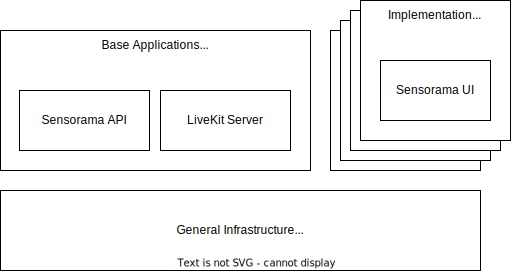
\includegraphics[scale=0.5]{04_Artefakte/01_Abbildungen/sensorama-stack}
\caption[Sensorama stack diagram]{The main components comprising the application architecture\protect}
\label{fig:sensoramaStack}
\end{figure}

Due to the containerised packaging and deployment, the application can be deployed in any cloud environment or other hosting platform providing virtual or dedicated hosts with root access.
The underlying software infrastructure requirement is minimal, and the required components are a Linux \ac{OS} with installations of Docker (with ContainerD) and Kubernetes.
No special hardware is needed, and the system can run in any environment that provides network access, storage space and standard computing resources.

While all the frameworks presented in \autoref{fig:mostUsedFrameworks} could be used to build an application as envisioned in this study, Vue was selected due to the relatively high acceptance and the comparably easy learning curve.
While it might not be the choice for large-scale or enterprise apps, the low entry barrier and the simple structure make it ideal to get an app up and running quickly, experiment with it and pass it on to others for hacking and custom modifications.
The Quasar framework was used to accelerate and simplify the initial development.
It extends Vue\textquotesingle s basic functionality with a \ac{UI} library complete with layout tools, common interface elements and a comfortable development and deployment environment.

The choice for a backend framework landed on Feathers and, by extension, Koa.
The simple structure and code generators allow for a speedy setup and deployment of a simple WebSockets \ac{API} that provides authentication and resource management.
It was connected to a MongoDB database because there was no definitive initial plan for how the stored and retrieved resources would be structured and typed.
Using a flexible document store, the data could be easily overwritten with updates and then wiped before the schema would eventually be deemed stable.

LiveKit was chosen as the WebRTC server implementation because it is versatile, and there is an easy installation method to set it up as a container running alongside the Redis database in Kubernetes.
While Mediasoup might have allowed a more precise implementation and probably a more efficient one, the workload overhead for building everything already offered by LiveKit was deemed too much effort for this kind of application.

\section{Design paradigms}
\label{sec:design-paradigms}

The basic design paradigm chosen for the Sensorama application was that of an \ac{SPA}.
As a remote API was already involved in managing access to shared resources, the extended \ac{PWA} paradigm was not helpful for this scenario.
It was designed as an exclusively real-time application that uses WebSockets for all transmission between app components and uses the WebRTC standard for user communication.
The project was structured as a monorepo, where all components are developed across different languages in a single repository.

The application\textquotesingle s custom part was partitioned into the user interface, which was deployed as a static built \ac{HTML}/\ac{CSS}/\ac{JS} bundle, the \ac{API}, which was set up as a single-process Node.js application and the so-called \textquote{Data-Producers}, which are external native utilities written in Python and C++ that provide bridges to motion capture hardware.

The primarily favoured coding paradigm was \ac{OOP}, but this was not strictly enforced for all components.
As some frameworks prefer different, more functional paradigms that are also compositional (Vue) or aspect-oriented (Feathers), it was deemed beneficial to refrain from enforcing a singular coding style.
While this might usually be considered bad practice in terms of maintainability for long-term development, it served the purpose of a modular and somewhat transient \textquote{single-use} application structure.

An essential part of the development concept was the sequence of development phases.
As there was no explicit definition beforehand, the development started by establishing a functional skeleton first and worked within that to carve out the actual functionality.
Initially, monolithic large blocks of code were built.
Various approaches to desired functionality were quickly tried and discarded or kept and subsequently extracted into separate components grouped by functional association.
Using this strategy, it was essential to review and refactor regularly and often to solidify the application structure and prevent it from dissolving into \textquote{spaghetti code} and to avoid unnecessary side-effects among the components.
The core features were extracted into a separate \ac{SDK} module towards the end of the development process, and appropriate unit tests were written.
As the application could now move into practical testing and, thus, some sort of \textquote{production} deployment, the core functionality needed to become more rigid and covered by test cases.

The general user interface and data producers were considered transient because they served only the singular use case and should be subject to frequent future modifications.
These application components should be hackable and replaceable, so they were not formally tested, at least in the scope of this study.
The unit testing focused on the data input and output for the core functionality to provide a stable foundation by keeping all components connected in a unified messaging system.
By modelling the basic request and response cases and formulating them as tests, potential later users would also have a tangible way of understanding the application's core mechanics.

For \ac{JS}, three popular testing frameworks are Jest, Mocha, and Jasmine (\ref{tab:githubTestingFrameworks}), among others, that can be used for implementing unit testing for the project.
In this case, the selection skipped the most popular option of Jest in favour of Mocha, which is used by the Feathers \ac{API} framework in its generator for boilerplate code.
This way, basic tests to base work on were already available and, to keep the project consistent across modules were adopted for the core \ac{SDK} module as well.

\begin{table}[ht]
\centering
\caption{Popular JavaScript testing frameworks}
\label{tab:githubTestingFrameworks}
\begin{tabular}[t]{|l|r|}
\toprule
Framework & Stars on GitHub (k)\\
\midrule
\cite{githubJest} & 43.2\\
\cite{githubMocha} & 22.4\\
\cite{githubJasmine} & 15.7\\
\bottomrule
\end{tabular}
\end{table}


\section{Movement quality extraction}
\label{sec:movement-quality-extraction}

One quality chosen was the \textquote{average velocity}, generally defined as the distance travelled over time (e.g.\ m/s).
Additionally, two more specialised concepts, developed for expressive movement analysis, were selected: \textquote{Quantity of Movement}~\parencite[96-97]{movementQualities}, describing the amount of difference between poses over time, and the \textquote{Contraction Index}~\parencite[97]{movementQualities} which observes the density of space used by a pose.
While the former is easily defined as the velocity calculated for a singular point (the centre of mass with an equal distribution), the latter two have been initially developed to observe pixelated \ac{2D} camera images and needed to be translated to \ac{3D} space.

\section{Sonification method and sound spatialisation}
\label{sec:sonification-method-and-sound-spatialisation}

The three basic movement qualities extracted provided the basis for a reference pipeline implementing parameter mapping sonification (see \autoref{sec:movement-data-sonification}).
The movement qualities were made available to the application, enabling an event-based system where thresholds that switch a boolean value at the crossing time can be defined.
As these values are watched, events can be triggered depending on their on- or off-state.
At the time of an event, the current value of a quality or a combination of them can be used to determine the magnitude of the event\textquotesingle s impact.

A simple system of scales, chords, and note selection was introduced to create an example sonification algorithm.
The system was based on selecting a specific scale (e.g.\ E-minor) for which a list of possible chords could then be produced.
Each time an event is triggered on one of the qualities (e.g.\ Quantity of Movement), the actual value can be used to decide which chord to select from the list using the normalised value.
The notes selected from the chord are then transposed using another quality (Contraction Index), selecting the root note for the chord across the octaves.
The average velocity was used to set the note length, triggering shorter notes when standing relatively still and more extended notes while travelling in space.
It must be noted that while this is a valid example for a parameter mapping sonification and will produce largely harmonic notes, it falls short of producing an output of a more complex musical quality because it lacks the ability to construct deeper structures and dramaturgic variance.
However, if engaged over a more extended period and practised, it could still yield interesting results, but this would also require a very specific way of composing the movement required to produce musically exciting results.

Sound spatialisation was achieved by playing the notes through a panner node provided by the audio framework and the WebAudio \ac{API}.
Both the audio stream retrieved from the \ac{WebRTC} connection was connected to a panner node, and the sound produced from the synthesiser nodes for the local and remote participants.
If the participant's head orientation and position were available through motion capture or the head tracking device, this spatial information would also be applied to the listener node and the other spatial audio nodes.

\section{Messaging}
\label{sec:messaging}

Standards-compliant protocols enabled streamlined messaging among the disparate application components based on different languages and run in various environments (see \autoref{fig:messagingFlow}).
Starting on the client side, the motion capture data producer starts a local WebSockets server to which the web application running in the browser can connect and receive live data.
The browser application can connect to the custom head-tracking device using the WebBluetooth standard and receive data messages using the \ac{GATT}\footnote{\url{https://www.bluetooth.com/bluetooth-resources/intro-to-bluetooth-gap-gatt/}}.

The conferencing functionality implemented in the web application was used to send local microphone audio and to relay the local producer utilities\textquotesingle data to other participants via the LiveKit server using the WebRTC protocol.
In the backend, the LiveKit server can push status updates as \ac{HTTP} webhook calls to the \ac{API} server to notify it about connects and disconnects.
The \ac{API} server uses the WebSockets protocol to relay updates on persisted data and LiveKit update events to the client browser and receives authentication and general data requests.

\begin{figure}[h]
\centering
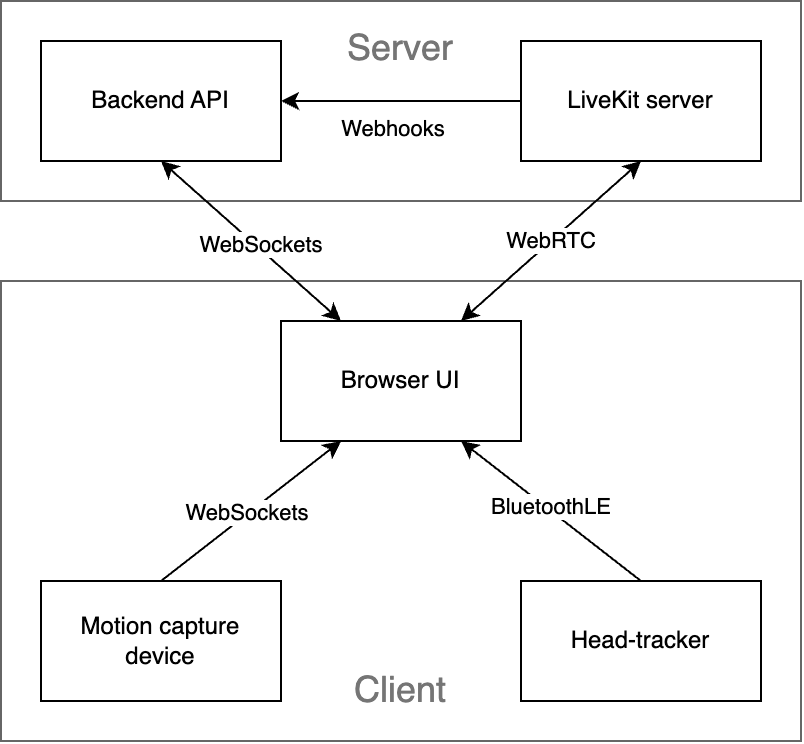
\includegraphics[scale=0.4]{04_Artefakte/01_Abbildungen/application-messaging-flow}
\caption[Application messaging flow]{Messaging flow between the application's components\protect}
\label{fig:messagingFlow}
\end{figure}

\section{Data modeling}
\label{sec:datamodeling}

Four core data models were defined for the application (see \autoref{fig:apiDataModel}).
The two models persisted by the \ac{API} server are \emph{Spaces} and \emph{Users}.
These were modelled as simple reference objects providing the basis for connecting users to virtual spaces, akin to spatial chat rooms, and each User can own multiple Space objects.
A Space is a container object representing a shared space populated with multiple participants\textquotesingle sensor readings.
Users can request one or more \emph{Token} objects that allow them to connect to a \textquote{room} on the LiveKit server that maps to a specific ID of a Space.
Once connected, the LiveKit server notifies the \ac{API} server of the new connection, and now the connected User\textquotesingle s ID can be found in the list retrieved from the virtual \textquote{connected} property of the Space object.

\begin{figure}[h]
\ centring
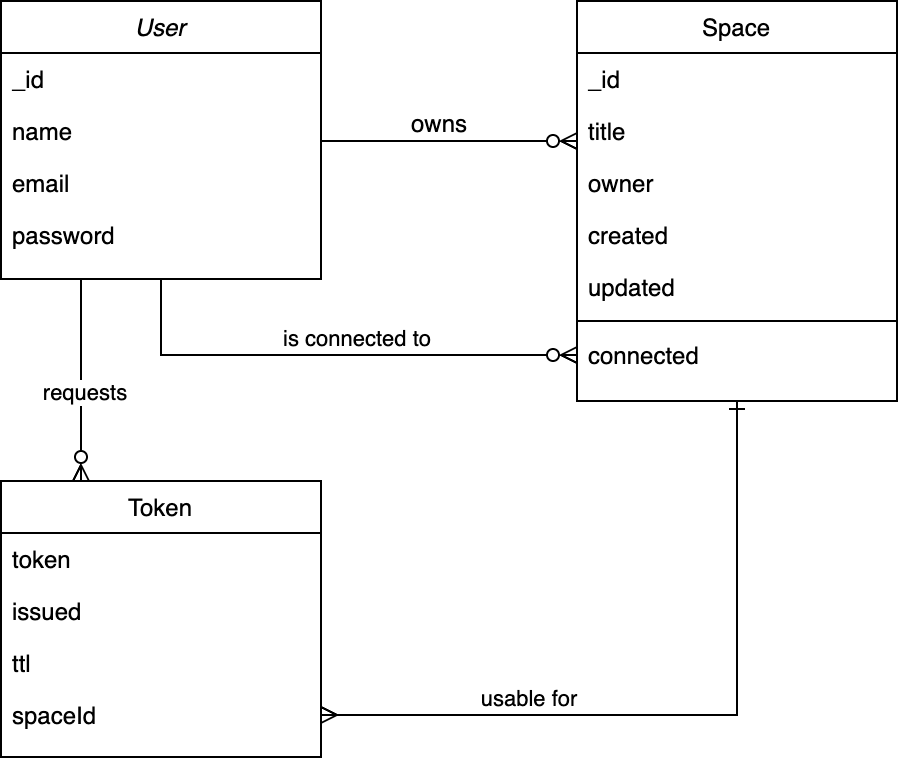
\includegraphics[scale=0.4]{04_Artefakte/01_Abbildungen/api-datamodel}
\caption[API data model]{Basic data model used in API server\protect}
\label{fig:apiDataModel}
\end{figure}

The connected participants can exchange arbitrary \emph{data messages}.
The data messages were not designed to be encoded as \ac{JSON} text messages but sent as raw data to make them as small as possible.
Messages were structured as byte sequences, with a 64bit long integer timestamp using the first eight bytes, then a single byte with an unsigned integer for selecting a message schema from the enumerated message types and a freely defined sequence of different number types (\autoref{fig:messageStructure}).
32-bit floating point numbers were used for all sensor readings as the numbers stay sufficiently small, and the precision is enough for millimetre measurements, statistical values or angles.
The numeric values were encoded in \ac{LE} format~\parencite{cohenEndianess} that appeared consistent across all environments but should be explicitly adhered to if other components were to be added to the application.

\begin{figure}[h]
\centering
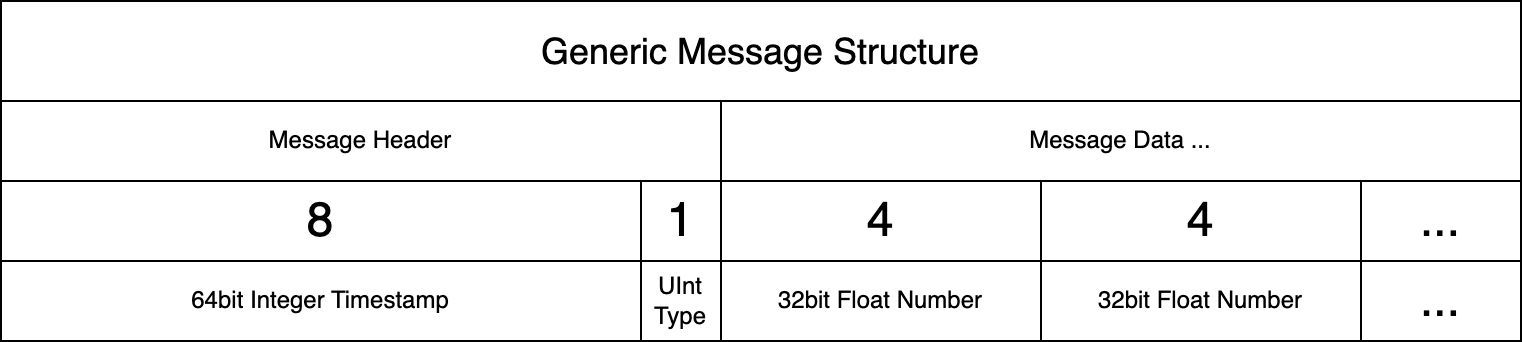
\includegraphics[width=\textwidth]{04_Artefakte/01_Abbildungen/generic-message-structure}
\caption[Generic Message Structure]{The basic message structure for transmitting numeric sensor readings\protect}
\label{fig:messageStructure}
\end{figure}

The message schemata were described in \ac{JSON} files to make them available across languages.
Shown in \autoref{listing:exampleMessage} is a simple example message schema for a nanosecond timestamp (\emph{{t\_ns}}), \emph{type} and one or more \ac{3D} \emph{points} stored as floats.

The root object\textquotesingle s property names resolve to the key under which the value could later be accessed.
The \emph{index} property specifies the byte index in the message, and \emph{count} specifies if the value repeats in sequence or is singular. \emph{dims} defines the dimensions for the value (e.g. \textquote{3} for a \ac{3D} point).
The \emph{type} could be a \textquote{Uint8}, \textquote{Float32} or a \textquote{BigInt64} and the property \textquote{le} specifies if this value is encoded as \ac{LE}.

\begin{listing}[!ht]
\inputminted{json}{04_Artefakte/03_Listings/example-pose-message.json}
\caption{Example pose message schema}
\label{listing:exampleMessage}
\end{listing}

\section{Application components}
\label{sec:application-components}

The application comprises several third-party components merely deployed as-is (WebRTC, databases, static web server) and the custom-developed parts described in the following section.

\subsection{Core SDK module}
\label{subsec:core-sdk-module}

The core functionality was built into a separate module to enable integration into other setups using different frameworks or architectures.
The module uses the \ac{NPM}\textquotesingle s package format and can be utilised in the browser and Node.js.
While this module carries the most fundamental functionality, it was created last in the development process, as the essential parts only crystallised during the initial development phase.

\subsection{Web frontend}
\label{subsec:web-frontend}

The web frontend provides the main entry point for the users.
It allows authentication via a local username and password combination and provides objects modelled as virtual \textquote{spaces} that are the central anchor to organise all communications, as defined in \autoref{fig:apiDataModel}.
Users can create spaces, name them and then join them, becoming active data producers, or choose to view them as passive spectators.

Depending on the participant\textquotesingle s role, a space is rendered as a different set of components.
Participants who actively join have access to a LocalProducer and a HeadTracker component.
These components provide a direct link via WebSockets to the external data-producer utilities and a WebBluetooth connection to the custom head-tracking device built on Arduino.
Those who only view the space do so via a dedicated scene viewer component that brings together all incoming streams and signals.

The frontend was designed to coordinate the connections between the WebRTC server, the backend \ac{API} and the local utilities.
It also implements the various web standard \ac{API}s needed for sound, graphics and communication.

\subsection{API backend}
\label{subsec:api-backend}

In the backend, the \ac{API} server was tasked with managing the basic connecting objects (spaces and users), general authentication, and generation of access tokens for the LiveKit server.
Through its real-time implementation, it can notify connected clients of changes like other connecting users or updates to data.
The Feathers framework exports its own client library that is specifically generated for the current server configuration.
It can be directly integrated into Vue using a client adapter module that handles authentication and basic \ac{CRUD} operations.

\subsection{Native utilities}
\label{subsec:native-utilities}

Three different native utilities were additionally implemented.

The general \emph{data producer} was set up as a \ac{CLI} utility in Python, implementing various Python-specific extensions: the DepthAI framework\footnote{\url{https://github.com/luxonis/depthai}}, used to work with the Luxonis Oak-D line of \ac{3D}-cameras, Intel\textquotesingle s OpenVino\footnote{\url{https://github.com/openvinotoolkit/openvino}} for interacting with various \ac{ML} models for pose recognition or point-cloud extraction, Open3D~\parencite{open3DZhou2018} for working with point cloud data and general spatial operations and PyMotion~\parencite{githubPyMotion}, a library for working with recorded \ac{BVH} motion capture data files.
Python also allowed for easy statistical data analysis using NumPy, which was used to perform movement quality extraction.

For real-time streaming of live motion capture data from the Captury Live system, there currently only exists a C++ client library provided by the system's manufacturer.
Thus, the \emph{Captury data producer} component had to be implemented separately and uses a C++-based WebSockets server streaming the library's received data.

As there was no affordable, open and platform-independent \emph{head-tracking} solution, this component was quickly prototyped using a BluetoothLE-ready Arduino device (Nano RP2040 Connect) and an \ac{IMU} component for absolute orientation measurement by Adafruit (9-DOF Absolute Orientation IMU Fusion Breakout) that can be directly connected to the Arduino using the \ac{I2C} serial bus.
The data read from the \ac{IMU} device is then posted as binary messages on a simple Bluetooth service.
The device could be directly integrated using the browser\textquotesingle s WebBluetooth web standard.

